% !TEX TS-program = xelatex
% !TEX encoding = UTF-8

\documentclass[11pt, a4paper]{article}

\usepackage{xltxtra} % loads fontspec and xunicode

\defaultfontfeatures{Mapping = tex-text, Scale = MatchLowercase}
\setmainfont{Adobe Garamond Pro}
\setsansfont{Helvetica}
\setmonofont{Bitstream Vera Sans Mono}

\usepackage{polyglossia}
% \setdefaultlanguage{austrian}
\setdefaultlanguage{german}

\usepackage{graphicx}

\usepackage{minted}
\definecolor{minted-bg}{rgb}{0.98, 0.98, 0.98}

\setlength\parindent{0mm}
\setlength\parskip{2mm}

\usepackage{url}

\usepackage{color}

\usepackage[pdfborder={0 0 0 0}]{hyperref}

\title{Unit-Tests für JavaScript und AJAX}
\author{Peter Krenn}

\begin{document}

\maketitle

\begin{abstract}
Zusammenfassung
\end{abstract}

\tableofcontents

\section{Einleitung}

Laut einer Umfrage\cite{young_dailyjs_2010} testen nur 34\% der Entwickler ihren
JavaScript Code. Im Vergleich zur vorjährigen Version der
Umfrage\cite{young_dailyjs_2009} gab es nur eine Verbesserung um 2\%. Trotzdem
existiert eine Vielzahl von JavaScript Testing Frameworks.

Die verbreitetsten Open Source JavaScript Frameworks und Libraries, wie zum
Beispiel jQuery\cite{resig_jquery_2011},
Prototype/Scriptaculous\cite{prototype_js_prototype_2011},
MooTools\cite{mootools_mootools_2011} oder YUI\cite{yahoo_inc._yui_2011-1}
verfügen alle über umfassende Test Suites.

Die von den JavaScript Frameworks verwendeten Test Frameworks sind auch die
am meisten eingesetzten: QUnit\cite{zaefferer_qunit_2011} (jQuery) 34\%,
Jasmine\cite{jasmine_jasmine_2011} (MooTools) 18\%,
YUITest\cite{yahoo_inc._yui_2011} (YUI) 6\%,
unittest.js\cite{fuchs_unittest.js_2011} (Prototype) 5\%.

Verbreitet ist weiterhin JsUnit\cite{jsunit_jsunit_2011} mit 12\%. Dieses
Framework war das erste JavaScript Unit Testing Framework und die Entwicklung
daran begann 2001, wurde aber mittlerweile eingestellt.

Neben Browser-basiertem Testen gewinnt Server-seitiges Testen an Bedeutung,
bereits 35\% der Entwickler verwenden JavaScript in einer Server Umgebung.
Node.js beinhaltet eine Implementierung der CommonJS Assertion Testing
Spezifikation\cite{node.js_node.js_2011}.

Ebenfalls für Server-seitiges Testen relevant sind Headless Testing Frameworks,
wie zum Beispiel Jasmine. Sie sind nicht vom DOM-Modell des Browsers oder
anderen Frameworks abhängig und können auch von der Kommandozeile aus aufgerufen
werden.

Auch Mocking und Stubbing Libraries wurden für JavaScript entwickelt.
Zum Beispiel Sinon.JS\cite{johansen_sinon.js_2011} funktioniert mit jedem Unit
Testing Framework und erlaubt es verschiedene Arten von Test Doubles und Fake
XHR Requests zu erzeugen.

Der weitere Artikel wird sich vor Allem mit der Anwendung von QUnit und Jasmine
beschäftigen. Diese beiden Test Frameworks sind die, an denen zur Zeit am
aktivsten entwickelt wird.

\section{QUnit}

QUnit\cite{zaefferer_qunit_2011} wird von Mitgliedern des jQuery
Teams\cite{resig_jquery_2011} entwickelt und ist auch die offizielle
\emph{test suite} des jQuery Projektes. Es zählt zur Gruppe der
xUnit Test Frameworks\cite{fowler_xunit_2010}, die einem Design folgen,
das erstmals mit SUnit\cite{beck_simple_1994} für Smalltalk formuliert
wurde und als JUnit\cite{gamma_junit_2011} für Java große Verbreitung fand.

\subsection{Assertions}

Der zentrale Bestandteil eines \emph{unit tests} ist die Assertion. Eine
Assertion ist eine Aussage über den Zustand einer bestimmten Stelle in
einem Programm\cite{wikipedia_assertion_2011}. Der Entwickler macht eine
Zusicherung, dass eine bestimmte Bedingung unabhänging von den Laufzeitumständen
immer wahr ist.

QUnit stellt eine Reihe von allgemeinen Assertions zur Verfügung,
die JUnit nachempfunden sind, und auch solche, die speziell an JavaScript
und asynchrone Entwicklung angepasst sind\cite{zaefferer_qunit_2011}:

\subsubsection*{\texttt{ok(state, message)}}

\texttt{ok()} ist eine boolsche Assertion, die positiv terminiert, wenn der
erste Parameter wahr ist. Den zweiten, optionalen Parameter \texttt{message} haben alle
Assertion-Funktionen gemein: dieser wird gemeinsam mit dem Ergebnis
ausgegeben.

\begin{minted}[gobble = 2, bgcolor = minted-bg]{javascript}
  ok(true, "terminiert immer positiv");
  ok("", "Leerstring entspricht false, die assertion schlägt fehl");
\end{minted}

\subsubsection*{\texttt{equal(actual, expecteded, message)}}

Diese Assertion ist \texttt{ok()} sehr ähnlich, allerdings werden die
\texttt{actual} und \texttt{expecteded} Werte mit dem Ergebnis ausgegeben. Dadurch
werden die Tests aussagekräftiger und \emph{debugging} einfacher.
\texttt{equal} terminiert positiv, wenn \texttt{actual == expecteded}. 

\begin{minted}[gobble = 2, bgcolor = minted-bg]{javascript}
  var actual = 1;
  equal(actual + 1, 2, "terminiert positiv");
  equal(actual, 2, "schlägt fehl");
\end{minted}

\subsubsection*{\texttt{strictEqual(actual, expected, message)}}

Im Gegensatz zu \texttt{equal()} werden bei dieser Assertion die Werte
mit \texttt{actual === expecteded} verglichen. Dieser Operator vergleicht
zusätzlich die Typengleichheit der beiden Parameter.

\begin{minted}[gobble = 2, bgcolor = minted-bg]{javascript}
  var actual = 0;

  // terminiert positiv, da == den Datentyp ignoriert
  equal(actual, false);

  // schlägt fehl, da 0 vom Typ Number und false Boolean ist
  strictEqual(actual, false);
\end{minted}

\subsubsection*{\texttt{deepEqual(actual, expected, message)}}

\texttt{deepEqual()} überprüft primitve Datentypen, Arrays und Objekte
rekursiv auf Gleichheit. Sie ist dabei auch strikter als \texttt{equal()}, da
der \texttt{===} Operator verwendet wird.

\begin{minted}[gobble = 2, bgcolor = minted-bg]{javascript}
  var actual = {a: 1};

  // equal schlägt mit verschiedenen Objekten fehl
  equal(actual, {a: 1});

  // schlägt fehl, da die Datentypen verschieden sind;
  deepEqual(actual, {a: "1"});

  // terminiert positiv, da die Inhalte der Objekte gleich sind
  deepEqual(actual, {a: 1}
\end{minted}

\subsubsection*{\texttt{notEqual(actual, expected, message)}}

Diese Assertion ist die invertierte Version von \texttt{equal()}.
Entsprechende Funktionen existieren auch für \texttt{strictEqual()} und
\texttt{deepEqual()}: \texttt{notStrictEqual()} und \texttt{notDeepEqual}.

\begin{minted}[gobble = 2, bgcolor = minted-bg]{javascript}
  var actual = 0;
  notEqual(actual, false, "schlägt fehl");
  notStrictEqual(actual, false, "terminiert positiv");

  var actual = {a: 1};
  notDeepEqual(actual, {a: "1"}, "terminiert positiv");
\end{minted}

\subsubsection*{\texttt{raises(state, message)}}

\texttt{raises()} überprüft, ob die übergebene \emph{callback} Funktion eine
\emph{exception} wirft. Die Funktion wird ohne Parameter im \emph{default scope}
aufgerufen.

\begin{minted}[gobble = 2, bgcolor = minted-bg]{javascript}
  raises(function() {
    throw new Error("Fehlerfall");
  }, "terminiert positiv, falls der gewünschte Fehler auftritt");
\end{minted}

\subsection{Testfunktionen}

Werden die vorgestellten Assertions direkt ausgeführt, unterbrechen sie
im Falle eines Fehlers den Testdurchlauf. Deswegen werden sie in Testfunktionen
eingebettet.

Es ist auch üblich, dass jede Testfunktion nur eine spezifische Eigenschaft
testet. Dies geschieht oft mit mehreren Assertions und die Testfälle
bleiben dabei überschaubar und einfach zu verstehen.

QUnit macht das mit der Funktion \texttt{test(name, expected, test)}.
\texttt{name} ist eine Bezeichnung des Tests und \texttt{test} ist eine
Funktion, die die Assertions enthällt. \texttt{expect} ist optional und
erlaubt es die Anzahl der zu erwartenden Assertions festzulegen. Dies ist
bei asynchronen Tests von Bedeutung.

\begin{minted}[gobble = 2, bgcolor = minted-bg]{javascript}
  Beispiel
\end{minted}

\subsection{Test Suites}

Mit der \texttt{module(name, lifecycle)} Anweisung ist es möglich, die Testfälle
weiter in Module aufzuteilen. Dies dient einerseits der Strukturierung der Tests
und andererseits wird es auch möglich, für mehrere Testfälle relevante Daten vor
deren Ausführung zu definieren.

\begin{minted}[gobble = 2, bgcolor = minted-bg]{javascript}
  Beispiel
\end{minted}

Im Parameter \texttt{lifecycle} kann man optional die Funktionen
\texttt{setup()} und \texttt{tearDown()} übergeben, die vor beziehungsweise nach
jedem Test ausgeführt werden. Sie teilen den \texttt{this}-\emph{scope} der
Testfunktionen, wodurch sogenannte \emph{fixtures} erstellt werden können. Die
Daten werden nach jedem Test zurückgesetzt, was in \texttt{tearDown()} auch
manuell geschehen kann.

\subsection{Asynchrones Testen}

Asynchrone Funktionen, wie sie bei AJAX Requests und Aufrufen von
\texttt{setTimeout()} und \texttt{setInterval()} vorkommen, können mit den
bisher vorgestellten Methoden nicht getestet werden.

Im folgenden Beispiel\cite{huang_how_2010} wird die Assertion nicht ausgeführt, da das
Ergebnis des Testfalles zum Zeitpunkt des Aufrufens bereits feststeht.

\begin{minted}[gobble = 2, bgcolor = minted-bg]{javascript}
  test("Asynchroner Test", function() {
    setTimeout(function() {
      ok(true);
    }, 100)
  });
\end{minted}

QUnit stellt aus diesem Grund zwei Funktionen zur Verfügung, mit der
sich der Testablauf pausieren und fortsetzen lässt.

\begin{minted}[gobble = 2, bgcolor = minted-bg]{javascript}
  test("Asynchroner Test", function() {
    stop();

    setTimeout(function() {
      ok(true);

      start();
    }, 100)
  })
\end{minted}

\texttt{stop()} hält den Test an und nach Aufrufen der Assertion, wird
mit \texttt{start()} wieder fortgesetzt. Da der Fall, dass \texttt{stop()} am
Anfang eines Tests ausgeführt wird, häufig vorkommt, gibt es dafür auch ein
spezielle Funktion names \texttt{asyncTest()}.

Wird nicht ein \texttt{setTimeout()} Aufruf sondern ein AJAX Request
getestet, bei dem man sich nicht sicher sein kann, wann und ob die
\emph{callback} Funktion ausgeführt wird, ist es möglich der \texttt{stop()}
Funktion ein Intervall als Paramter mitzugeben, nachdem der Testablauf
automatisch fortgesetzt wird. Der betreffende Test schlägt dabei fehl.

Werden in einem Testfall mehrere zeitverzögerte Aufrufe getestet, ist es
notwendig, \texttt{start()} manuell mit \texttt{setTimout()} ausreichend zu
verzögern, so dass alle \emph{callbacks} ausreichend Zeit zum Terminieren haben.

Um sicher zu stellen, dass alle \emph{callbacks} mit den enthaltenen
Assertions ausgeführt werden, gibt es eine \texttt{expect()} Funktion,
der man als Parameter die zu erwartende Anzahl der Assertions übergeben
kann.

\begin{minted}[gobble = 2, bgcolor = minted-bg]{javascript}
  // Ein AJAX request mit der zu testenden callback Funktion
  function ajaxCall(successCallback) {
    jQuery.ajax({
      url: "http://server.com/",
      success: successCallback
    });
  }

  asyncTest("Asynchroner Test", function() {
    // asyncTest unterbricht den Testablauf

    // 3 assertions sollten ausgeführt werden
    expect(3);

    ajaxCall(function() {
      ok(true);
    });

    ajax(function() {
      ok(true);
      ok(true);
    })

    // Nach 3000 ms wird der Testablauf fortgesetzt
    setTimeout(function() {
      start();
    }, 3000);
  });
\end{minted}

Die Kombination von \texttt{expect()} mit \texttt{asyncTest()} ist wiederum so
verbreitet, dass die Anzahl der zu erwartenden Assertions als zweiter
Parameter direkt in den \texttt{asyncTest()} Aufruf verlegt werden kann.

JQuery stellt dafür die Methoden \texttt{stop()} und \texttt{start()}

\subsection{Testablauf}

Die Ausgabe von QUnit erfolgt ausschließlich im Browser. Die Dateien
\texttt{qunit.js} und \texttt{qunit.css} müssen gemeinsam mit dem zu testenden
JavaScript Code und den Tests in eine HTML-Datei eingebunden werden.

\begin{minted}[gobble = 2, bgcolor = minted-bg]{html}
  <!DOCTYPE html>
  <html lang="en">
    <head>
      <script type="text/javascript" src="qunit.js"></script>
      <link rel="stylesheet" href="qunit.css" type="text/css"
            media="screen" />

      <!-- project file -->
      <script type="text/javascript" src="my_project.js"></script>

      <!-- tests file -->
      <script type="text/javascript" src="my_tests.js"></script>
    </head>
    <body>
      <h1 id="qunit-header">QUnit example</h1>
      <h2 id="qunit-banner"></h2>
      <div id="qunit-testrunner-toolbar"></div>
      <h2 id="qunit-userAgent"></h2>
      <ol id="qunit-tests"></ol>
      <div id="qunit-fixture">test markup, will be hidden</div>
    </body>
  </html>
\end{minted}

Beim Ausführen der Datei im Browser befüllt QUnit die Elemente im
\texttt{body} mit den Ergebnissen der Tests.

\begin{center}
  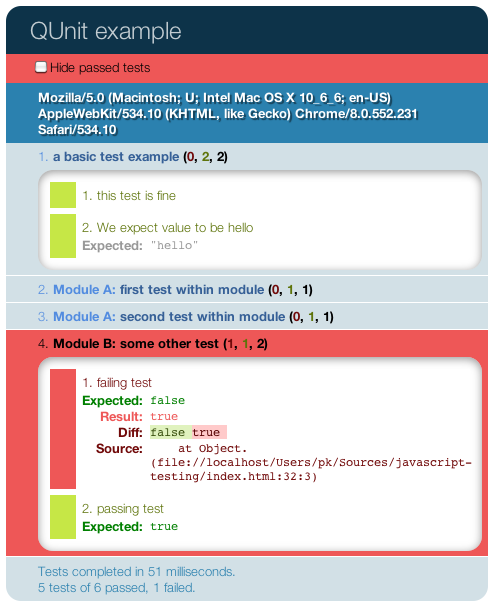
\includegraphics[width = 1\textwidth]{QUnit.png}
\end{center}

Für jeden Testfall wird die Anzahl der erfolgreichen und fehlgeschlagenen
Assertions und auch deren Gesamtanzahl angegeben. Für fehlgeschlagene
Tests wird dessen Position im Quellcode angezeigt.

QUnit ist nur für die Verwendung im Browser ausgelegt, ein
Kommandozeilen-basierter Aufruf der Testfälle ist nicht vorgesehen. Ein
Versuch\cite{plee_qunit_2010} QUnit in der simulierten Browserumgebung
Env.js\cite{resig_envjs_2011} anzuwenden, war nur begrenzt erfolgreich, da der
Testbericht im HTML-Format ausgegeben wird. Eine Alternative ist das weiter
unten beschriebene TestSwarm Projekt.

\section{Jasmine}

Jasmine\cite{jasmine_jasmine_2011} gehört zur Gruppe der Behavior Driven
Development\cite{wikipedia_behavior_2011} oder BDD Frameworks. Im Gegensatz zu
traditionellen xUnit Test Frameworks versuchen diese die Sprache, in der die
Tests verfasst sind, einfacher und damit auch für nicht-technische
Projektteilnehmer verständlich zu machen. BDD soll dabei helfen, die gewünschte
\emph{software behavior} in Diskussion mit den Auftraggebern klar zu definieren.

Im Gegensatz zu seinem Vorgänger Screw.Unit\cite{sobo_screw.unit_2011} und QUnit
ist Jasmine ein Headless Testing Framework, das heißt es benötigt keinen
Browser und ist nicht von anderen JavaScript Libraries abhängig. Dies
vereinfacht den automatisierten Aufruf der Tests und ermöglicht es Server-side
Anwendungen zu testen. Wie QUnit unterstützt es asynchrones Testen und verfügt
außerdem über Mocking und Stubbing Funktionalitäten.

\subsection{Specs, Expectations und Suites}

Specs entsprechen den Testfunktionen von klassischen xUnit Test Frameworks. Sie
beschreiben das Verhalten einer Funktion oder eines Objektes mit einem Aufruf
der Funktion \texttt{it()} in Form einer natürlichen Sprache. Die Beschreibung
sollte aussagekräftig sein, da sie im Testbericht ausgegeben wird.

Expectations drücken die Erwartungen an das Verhalten eines bestimmten Teils des
Quellcodes mittels der \texttt{expect()} Funktion aus. Sie sind vergleichbar mit
den Assertions der xUnit Frameworks. Das gewünschte Verhalten wird durch
Matchers wie \texttt{toEqual} spezifiziert:

\begin{minted}[gobble = 2, bgcolor = minted-bg]{javascript}
  it("should increment a variable", function() {
    // Definition der Testdaten
    var value = 0;

    // Ausführen des zu testenden codes
    value++;

    // Testen der Erwartung
    expect(value).toEqual(1);
  });
\end{minted}

Zur Strukturierung der Specs dienen Suites. Wie bei QUnit ist es möglich,
Anweisungen vor und nach dem Aufrufen jedes Tests auszuführen -- dies geschieht
mit \texttt{beforeEach()} und \texttt{afterEach()}.

\begin{minted}[gobble = 2, bgcolor = minted-bg]{javascript}
  describe("Calculator", function() {
    var a, b;

    beforeEach(function() {
      a = 3;
      b = 4;
    });

    it("should add numbers with add()", function() {
      expect(Calculator.add(a, b)).toEqual(7);
    });

    it("should multiply numbers with multiply()", function() {
      expect(Calculator.multiply(a, b)).toEqual(12);
    });
  });
\end{minted}

\subsection{Matchers}

Jasmine verfügt über eine Reihe von eingebauten Matchers und deren Inversionen,
die man durch Voranstellen von \texttt{.not} erhält:

\subsubsection*{\texttt{toEqual()}}

Dieser Matcher entspricht der QUnit Assertion \texttt{deepEqual()} und
kann außerdem Datumswerte und DOM-Nodes vergleichen.

\begin{minted}[gobble = 2, bgcolor = minted-bg]{javascript}
  // Alle expectations terminieren positiv
  expect(true).toEqual(true);
  expect(false).not.toEqual(true);

  expect("5").not.toEqual(5);

  expect({a: 1}).not.toEqual({a: "1"});

  expect(new Number("5")).toEqual(5);

  expect(new Date("January 11, 2011, 12:00:00"))
    .not.toEqual(new Date("January 12, 2011, 12:30:00"));

  var nodeA = document.createElement("div");
  var nodeB = document.createElement("div");
  expect(nodeA).toEqual(nodeA);
  expect(nodeA).not.toEqual(nodeB);
\end{minted}

\subsubsection*{\texttt{toBe()}}

\texttt{toBe()} entspricht \texttt{strictEqual()}.

\begin{minted}[gobble = 2, bgcolor = minted-bg]{javascript}
  var a = {};
  var b = {};
  var c = b;

  expect(a).not.toBe(b);
  expect(c).toBe(b);
\end{minted}

\subsubsection*{\texttt{toMatch()}}

\texttt{toMatch()} überprüft Strings auf Übereinstimmungen mit Regulären
Ausdrücken.

\begin{minted}[gobble = 2, bgcolor = minted-bg]{javascript}
  expect("javascript").toMatch(/script/);
  expect("javascript").not.toMatch(/testing/);
\end{minted}

\subsubsection*{\texttt{toBeDefined()}}

\texttt{toBeDefined()} terminiert positiv für definierte Werte.

\begin{minted}[gobble = 2, bgcolor = minted-bg]{javascript}
  var a = 5;

  expect(a).toBeDefined();

  expect(undefined).not.toBeDefined();
\end{minted}

\subsubsection*{\texttt{toBeNull()}}

\texttt{toBeNull()} erwartet einen \texttt{null}-Wert.

\begin{minted}[gobble = 2, bgcolor = minted-bg]{javascript}
  expect(null).toBeNull();
  expect(undefined).not.toBeNull();
\end{minted}

\subsubsection*{\texttt{toBeTruthy()} und \texttt{toBeFalsy()}}

Diese Matchers überprüfen, ob ein Ausdruck in \texttt{true} beziehungsweise
\texttt{false} evaluiert.

\begin{minted}[gobble = 2, bgcolor = minted-bg]{javascript}
  expect(0).not.toBeTruthy();
  expect("").toBeFalsy();
  expect(5).toBeTruthy();
  expect({a: 1}).not.toBeFalsy();
\end{minted}

\subsubsection*{\texttt{toContain()}}

\texttt{toContain()} terminiert positiv, falls der übergebene String oder Array
ein bestimmtes Zeichen oder Element enthält.

\begin{minted}[gobble = 2, bgcolor = minted-bg]{javascript}
  expect("javascript").toContain("a");
  expect("javascript").not.toContain("x");

  expect([1, 2, 3]).toContain(3);
  expect([1, 2, 3]).not.toContain("x");
\end{minted}

\subsubsection*{\texttt{toBeLessThan()} und \texttt{toBeGreaterThan()}}

Diese Matchers überprüfen, ob ein Wert kleiner beziehungsweise größer als der
Übergebene ist.

\begin{minted}[gobble = 2, bgcolor = minted-bg]{javascript}
  expect(5).toBeLessThan(10);
  expect(5).not.toBeGreaterThan(10);
\end{minted}

\subsubsection*{\texttt{toThrow()}}

Mit \texttt{toThrow()} drückt man die Erwartung aus, dass ein festgelegter
Ausdruck die übergebene Exception wirft.

\begin{minted}[gobble = 2, bgcolor = minted-bg]{javascript}
  expect(function() { throw new Error("error"); }).toThrow("error");
\end{minted}

\subsubsection*{Benutzerdefinierte Matchers}

Um die Lesbarkeit der Specs zu verbessern, ist es mit Jasmine auch möglich eigene
Matchers zu definieren. Eine Matcher Funktion erhält den zu vergleichenden Wert
als \texttt{this.actual} und es können zusätzlich beliebig viele Parameter
übergeben werden. Die benutzerdefinierten Matchers werden mit
\texttt{this.addMatchers()} in der \texttt{beforeEach()} oder der \texttt{it()}
Funktion definiert.

\begin{minted}[gobble = 2, bgcolor = minted-bg]{javascript}
  beforeEach(function() {
    this.addMatchers({
      toBeLessOrEqualThan: function(expected) {
        return this.actual <= expected;
      }
    });
  });
\end{minted}

\subsection{Asynchrones Testen}

Zum Testen von asynchronen Funktionen stellt Jasmine die Funktionen
\texttt{runs()}, \texttt{waits()} und \texttt{waitsFor()} bereit.

Von \texttt{runs()} aufgerufene Funktionen für sich alleine verhalten sich
genauso, als wären sie direkt aufgerufen worden. In Verbindung mit
\texttt{waits()} kann der Testablauf für eine bestimmte Zeit unterbrochen
werden, bis die nächste \texttt{runs()} Funktion aufgerufen wird. Die
\texttt{runs()} Blöcke innerhalb eines \texttt{it()} Blocks teilen den gleichen
\texttt{this}-\emph{scope}.

\begin{minted}[gobble = 2, bgcolor = minted-bg]{javascript}
  it("should increment a value after 250 ms", function() {
    runs(function() {
      this.value = 0;

      // 250 ms in der Zukunft wird value erhöht
      setTimeout(function() {
        this.value++;
      }, 250);
    });

    // value entspricht noch dem initialisierten Wert
    runs(function() {
      expect(this.value).toEqual(0);
    });

    waits(500);

    // 500 ms später wurde value korrekt erhöht
    runs(function() {
      expect(this.value).toEqual(1);
    });
  });
\end{minted}

\texttt{waitsFor()} pausiert den Testablauf, bis ein bestimmtes Ereignis
eintrifft. Als erster Parameter wird eine Funktion übergeben, die \texttt{true}
im Falle des Eintreffens des Ereignisses zurück gibt. Optional kann auch die
maximale Wartedauer und eine Fehlermeldung übergeben werden.

\begin{minted}[gobble = 2, bgcolor = minted-bg]{javascript}
  describe('Calculation', function() {
    it('should calculate a value asynchronously', function() {
      var calculation = new Calculation();
      calculation.asynchronouslyCalculateValue();

      // waitsFor() wartet bis isComplete() true zurück gibt
      // maximal aber eine Sekunde
      waitsFor(function() {
        return calculation.isComplete();
      }, "calculation wasn't completed", 1000);

      runs(function() {
        expect(calculation.value).toEqual(1);
      });
    });
  });
\end{minted}

\subsection{Spies}

Jasmine Spies sind Test Doubles\cite{meszaros_test_2011-1}, die als Stubs,
Spies oder in Verbindung mit einer Expectation als Mocks agieren können.
Test Doubles sind Objekte, die das Interface oder Verhalten eines realen
Objektes simulieren und werden eingesetzt um die Komplexität der Tests zu
reduzieren. Bei Projekten, die viele verschachtelte Objekte und Module umfassen,
macht es Sinn, sich beim Testen nur auf relevante Teile zu konzentrieren und bei
Kommunikation nur auf die korrekte Verwendung der Interfaces zu achten. Für
JavaScript relevante Beispiele sind asynchrone Aufrufe oder AJAX Requests.

Test Stubs sind Objekte, die ausschließlich auf die für den Test notwendigen
Aufrufe reagieren. Eine erweiterte Version sind Test Spies, sie zeichnen die
Anzahl und Parameter der Aufrufe auf, welche später in Assertions oder
Expectations getestet werden können. Mocks sind vordefinierte Objekte mit
eingebauten Expectations, die bestimmen welche Aufrufe erwartet werden.

\texttt{spyOn(object, methodName)} verhindert im ersten Schritt den Aufruf einer
Funktion und zeichnet folgende Eigenschaften auf: \texttt{callCount} enthält wie
oft die Funktion aufgerufen worde, \texttt{mostRecentCall.args} ist
Parameter-Array des letzten Aufrufes und mit \texttt{argsForCall[]} kann man auf
die Parameter sämtlicher Aufrufe zugreifen.

\begin{minted}[gobble = 2, bgcolor = minted-bg]{javascript}
  // Ein Objekt, dessen Interface simuliert wird
  var example = {
    not: function(boolean) { return !boolean; }
  };

  // Ein Spy wird für example.not angelegt
  spyOn(example, "not");
  example.not(true);

  // example.not.callCount: 1
  // example.mostRecentCall.args: [true]
\end{minted}

Im Falle eines Aufrufes kann die Reaktion eines Spies festgelegt werden:

\begin{minted}[gobble = 2, bgcolor = minted-bg]{javascript}
  // ruft die originale Funktion auf
  spyOn(example, "not").andCallThrough();

  // gibt die übergebene Werte bei Aufruf zurück
  spyOn(example, "not").andReturn(true);

  // wirft bei Aufruf eine Exception
  spyOn(example, "not").andThrow("error");

  // ruft die übergebene Funktion auf
  spyOn(example, "not").andCallFake(function() { return true; });
\end{minted}

Mit folgenden Matchers können die Spies in Expectations verwendet werden.
Dadurch verhalten sich die Funktionen als Mocks.

\begin{minted}[gobble = 2, bgcolor = minted-bg]{javascript}
  spyOn(example, "not");
  example.not(true);

  expect(example.not).toHaveBeenCalled();
  expect(example.not).not.toHaveBeenCalledWith(false);
\end{minted}

Anstatt eine bestehende Funktion zu einem Spy zu machen, ist es auch manchmal
sinnvoll, mit \texttt{jasmine.createSpy()} ein Stub-artiges Objekt manuell zu erstellen.
Ein Anwendungsgebiet ist das Testen von Callbacks\cite{jasmine_jasmine_2011-1}.

\begin{minted}[gobble = 2, bgcolor = minted-bg]{javascript}
  var Klass = function() {
  };

  Klass.prototype.methodWithCallback = function(callback) {
    return callback("example");
  };

  it("should spy on Klass#methodWithCallback", function() {
    var callback = jasmine.createSpy();
    new Klass().methodWithCallback(callback);

    expect(callback).toHaveBeenCalledWith("example");
  });
\end{minted}

Eine weitere Anwendung ist das Testen von AJAX Request oder asynchronen
Funktionen, die Callbacks als Parameter verlangen. Die Request beziehungsweise
die Funktion wird dabei nicht ausgeführt, sondern die Callback Funktion wird
isoliert getestet.

\begin{minted}[gobble = 2, bgcolor = minted-bg]{javascript}
  var Klass.prototype.asyncMethod = function(callback) {
    asyncCall(callback);
  };

  it("should test async call") {
    spyOn(Klass, 'asyncMethod');
    var callback = jasmine.createSpy();

    Klass.asyncMethod(callback);
    expect(callback).not.toHaveBeenCalled();

    // Die an asyncMethod übergebene callback Funktion
    // wird manuell getestet
    Klass.asyncMethod.mostRecentCall.args[0]("example");
    expect(callback).toHaveBeenCalledWith("example");
  });
\end{minted}

\subsection{Testablauf}

Für Jasmine gibt es eine Stand-alone Version, deren Funktionalität der von QUnit
entspricht. In einer HTML-Datei werden die Test-, sowie die Projektdateien
eingebunden und beim Öffnen im Browser wird sie mit den Testergebnissen befüllt.

\begin{center}
  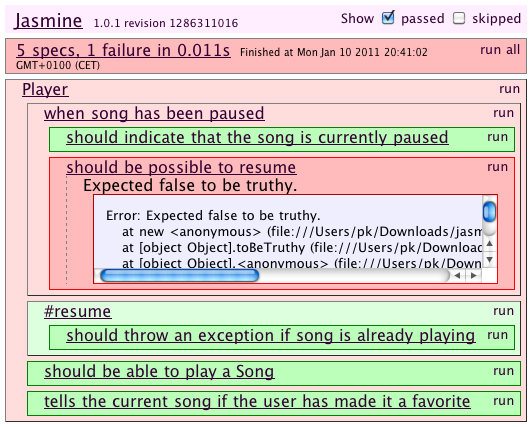
\includegraphics[width = 1\textwidth]{Jasmine.png}
\end{center}

Nicht erfüllte Expectations werden farblich markiert und der Stack für den
jeweiligen Fehler wird angezeigt. Zusätzlich ist es möglich, einzelne Specs vom
Browser aus erneut aufzurufen.

Mit dem Kommandozeilen Interface von Jasmine ist es möglich automatisiert
verschiedene Browser zu starten und die Test Suites auszuführen. Die Browser
werden von Selenium\cite{selenium_selenium_2011} geladen und geben die
Ergebnisse über die Kommandozeile aus.

Ein Beispiel für die Server-seitige Anwendung von Jasmine ist
jasmine-node\cite{hevery_jasmine-node_2011}, eine Adaptierung für node.js. Die
Specs können direkt mit dem node.js Interpreter ausgeführt und ausgegeben
werden.

\section{Regression Testing}

Regression Testing\cite{wikipedia_regression_2011} versucht Probleme und
Nebenwirkungen von Modifikationen im Quellcode durch Wiederholung der Testfälle
aufzuzeigen. Ein verwandter Begriff ist Continuous
Integration\cite{wikipedia_continuous_2011}, die kontinuierliche
Qualitätskontrolle für ein Projekt erreichen will. Automatisiertes Testing ist
eines ihrer Ziele. 

Da es keine einheitliche JavaScript Implementierung gibt, sondern
diese sich je nach Browser, Browserversion und Betriebssystem unterscheiden, ist
die Durchführung der Testläufe problematisch.

Ein Ansatz, der sich derzeit in Entwicklung befindet, ist
TestSwarm\cite{resig_testswarm_2011} von John Resig, dem Autor von jQuery und
QUnit. Es handelt sich dabei um ein System, das den Code eines Projektes bei
jedem \emph{commit} im Versionierungssystem automatisch auf verschiedenen
Plattformen und Browsern testet.

Das System wird von einem zentralen Server aus gesteuert, der Testaufträge an
mehrere Clients, auf denen verschiedene Browserversionen laufen, weiterleitet.
Das Ergebnis der Prozesses ist eine tabellarische Ansicht die für jeden
\emph{commit} darstellt, auf welchen Plattformen und Browsern die Test Suite
fehlerfrei angewendet worden ist.

Im Gegensatz zu vergleichbaren Systemen, wie
Selenium\cite{selenium_selenium_2011}, ist TestSwarm vom verwendeten Test
Framework unabhängig: es werden alle im Moment gebräuchlichen Frameworks
unterstützt.

\begin{flushleft}
  \bibliography{javascript-testing}
  \bibliographystyle{plain}
\end{flushleft}

\end{document}
